\input ../SlidePreamble
\input ../preamble


\begin{document}

{\Huge
  \centerline{\bf TTIC 31230,  Fundamentals of Deep Learning}
  \vfill
  \centerline{David McAllester, Winter 2020}
  \vfill
  \centerline{\bf  The Transformer}
  \vfill
  \vfill

\slide{The Transformer}

Attention is All You Need, Vaswani et al., June 2017

\vfill
The transformer has now essentially replaced RNNs in natural language applications.

\vfill
The recent progress on natural language understanding (GLUE) is based on general language modeling using transformers.

\slide{The Transformer}

Unlike RNNs, transformers run in parallel time in proportional to the layering depth
independent of the length of the input sequence.

\vfill
Transformers also do a better job of allowing information early in the sequence to be used later in the sequence --- they have better memory when used as a langauge model.

\slide{The Transformer}

\centerline{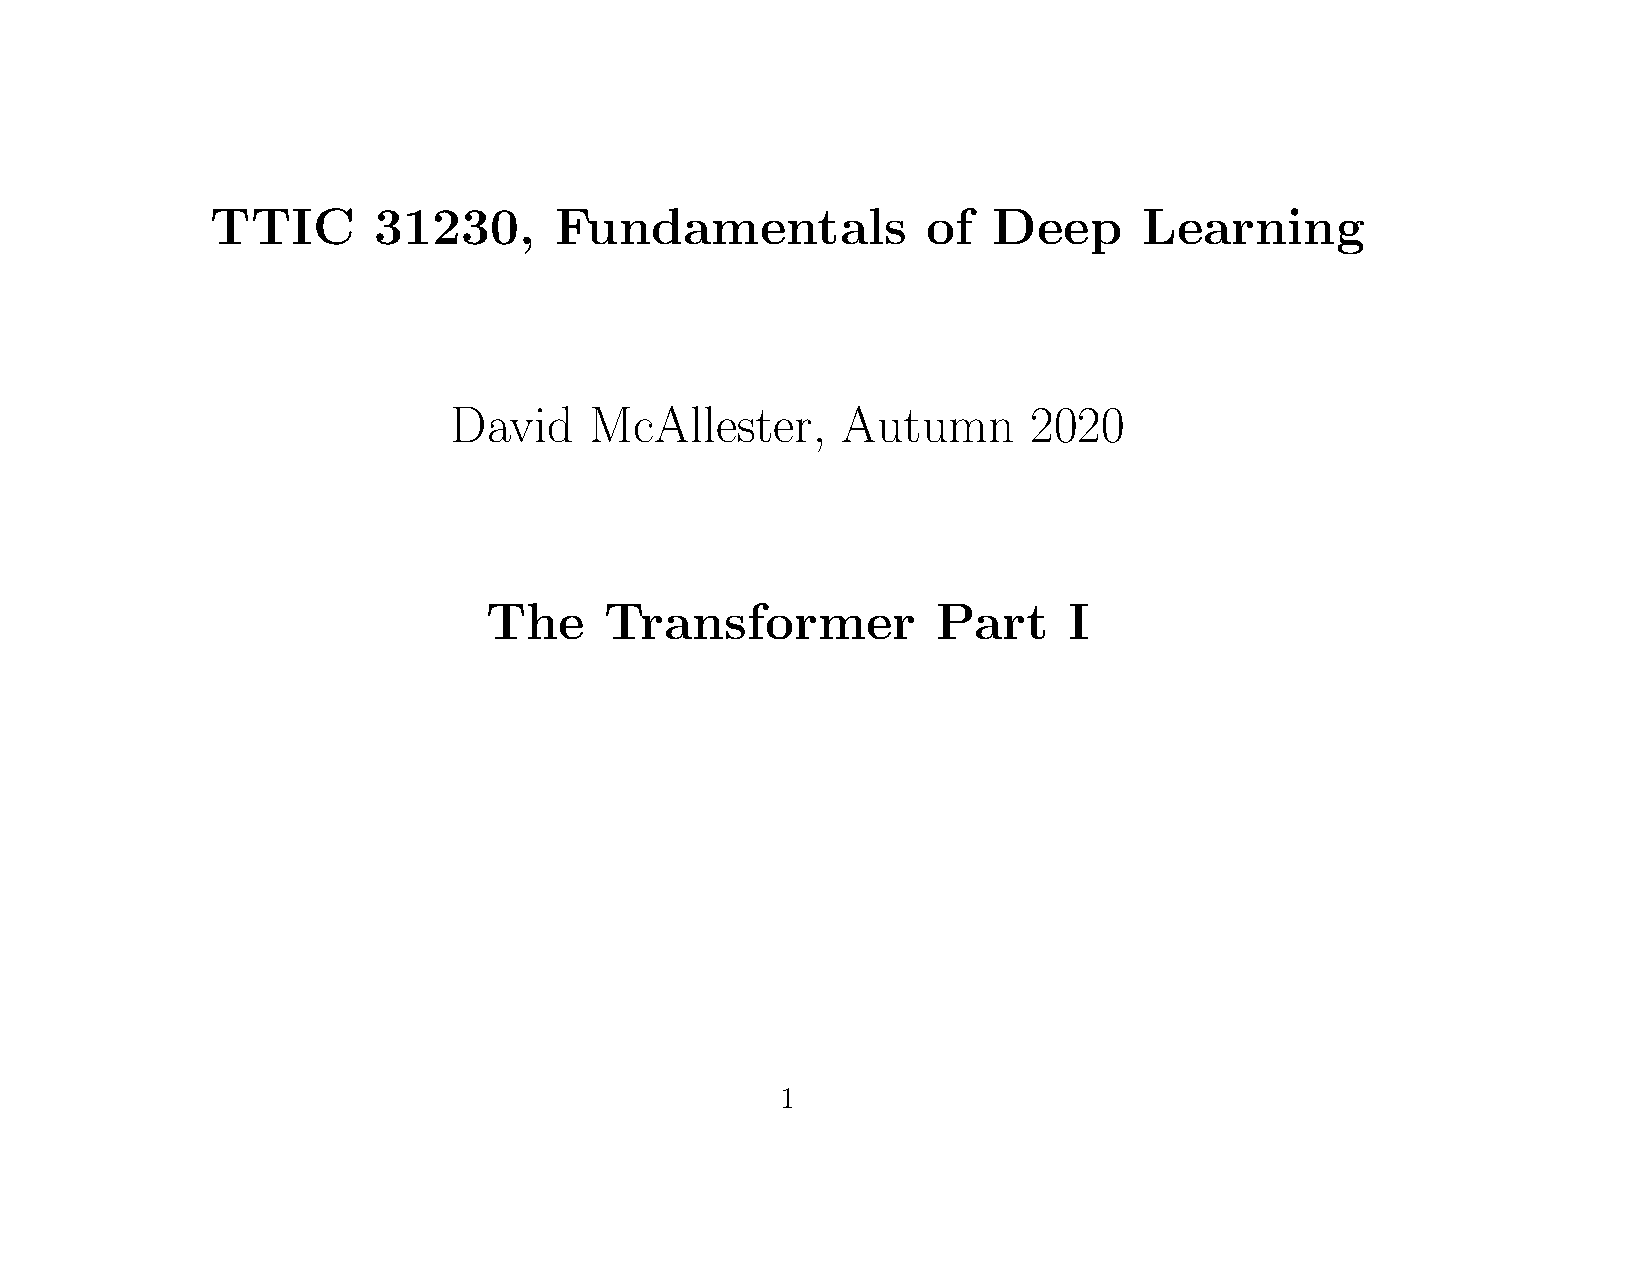
\includegraphics[height=4.5in]{\images/transformer}}

{\huge
\centerline{Jay Alammar's blog}
}

All layers run in $O(1)$ parallel time independent of text length.

\slide{The Transformer}

\centerline{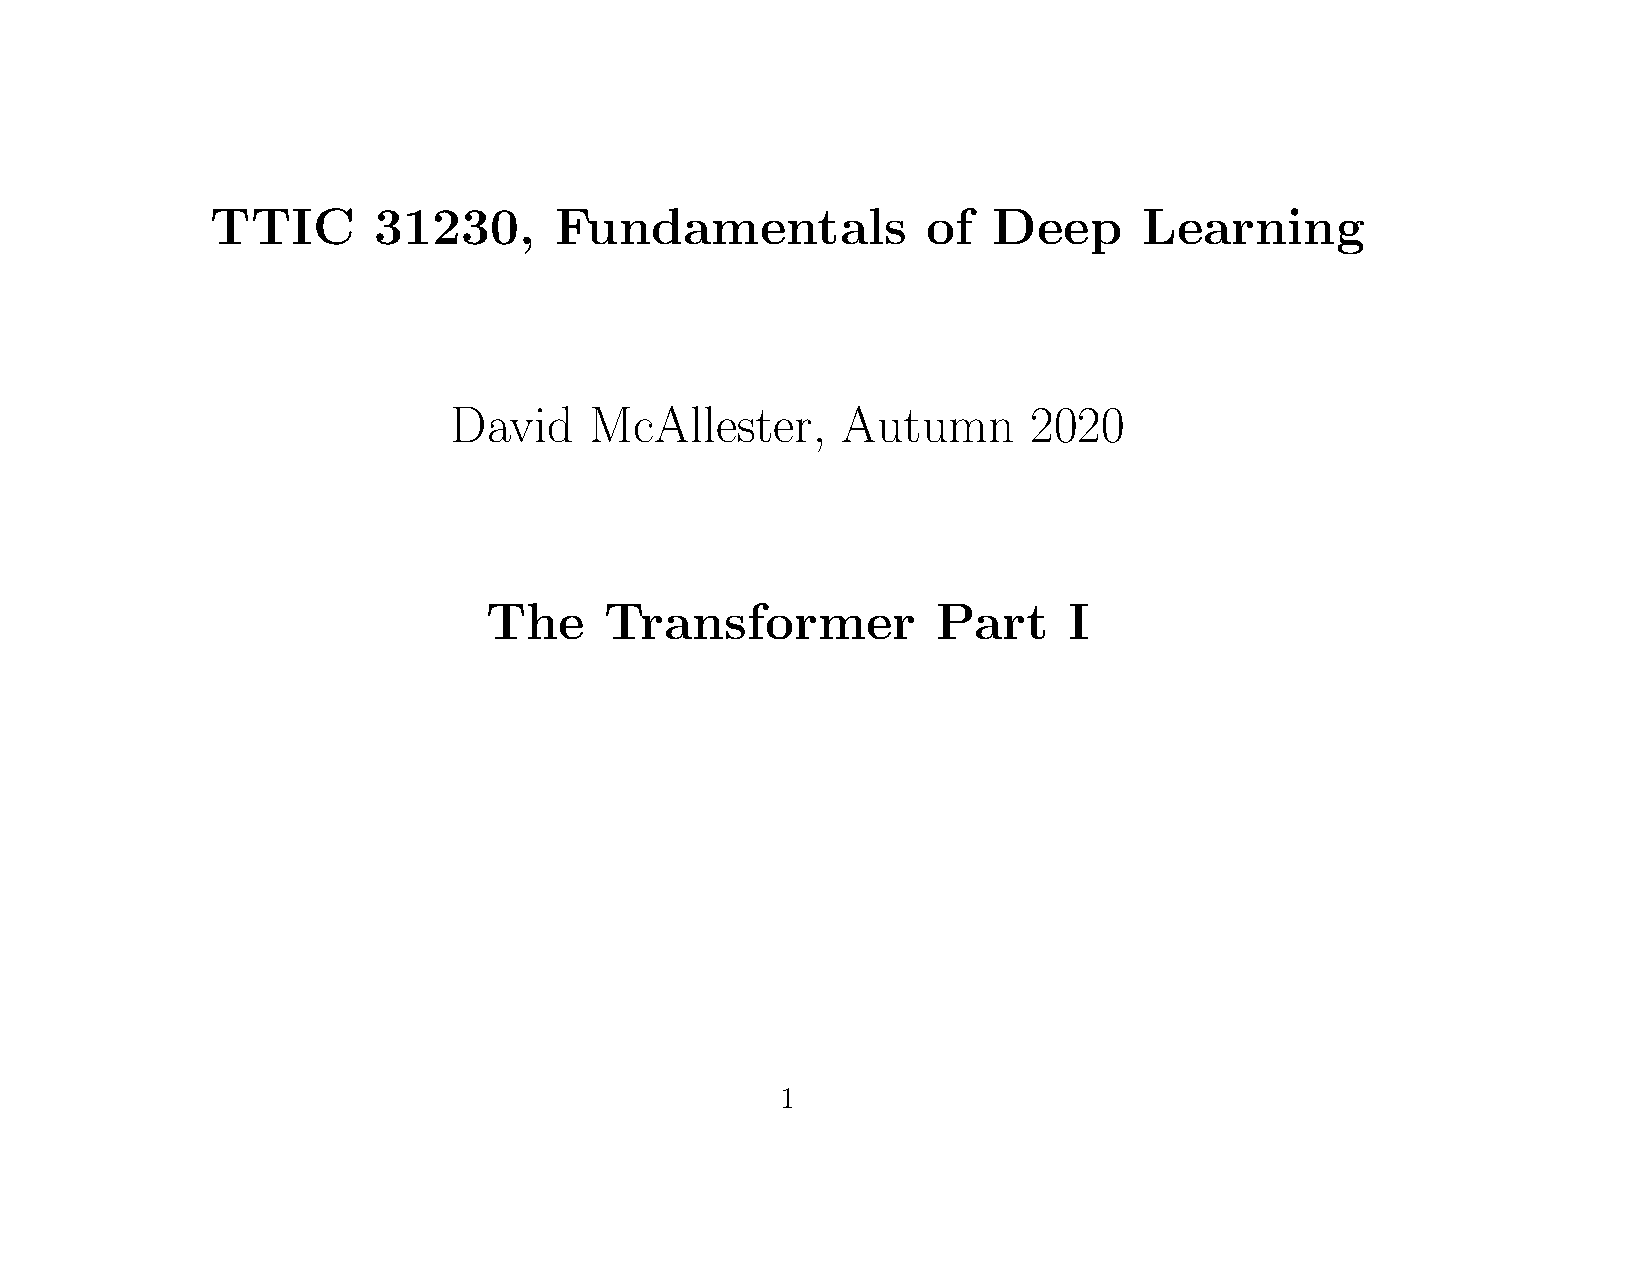
\includegraphics[height=4.5in]{\images/transformer}}

{\huge
\centerline{Jay Alammar's blog}
}

Layers are stacked with residual connections.

\slide{A Self-Attention Layer}

Given an $h_\mathrm{in}[T,J]$ we will construct $h_\mathrm{out}[T,J]$ (``in'' and ``out'' refer to layering, not translation).
\vfill

We first construct a head-specific self-attention $\alpha[k,t_1,t_2]$ --- the attention position
$t_1$ is giving to position $t_2$ for ``head'' $k$.

\vfill
The motivation for different heads is that there are different relationships between words such as ``refers to'' for pronouns,
or ``subject of'' and ``object of'' for verbs. But the meaning of each head is not specified and emerges from training.

\slide{Computing the Self Attention}

For each head $k$ and position $t$ we compute a key vector and a query vector with dimension $U$ typically smaller than dimension $J$.
      
\begin{eqnarray*}
\mathrm{Query}[k,t,u] & = & W^Q[k,u,J]h_\mathrm{in}[t,J] \\
\\
\mathrm{Key}[k,t,u] & = &  W^K[k,u,J]h_\mathrm{in}[t,J] \\
\\
\alpha[k,t_1,t_2] & = & \softmax_{t_2}\; \mathrm{Query}[k,t_1,U]\mathrm{Key}[k,t_2,U]
\end{eqnarray*}

\slide{Computing the Output}

We require $I = J/K$.
      
\begin{eqnarray*}
\mathrm{Value}[k,t,i] & = & W^V[k,i,J]h_\mathrm{in}[t,J] \\
\\
\tilde{h}_\mathrm{out}[k,t,i] & = & \alpha[k,t,T_2]\mathrm{Value}[k,T_2,i] \\
\\
h_\mathrm{out}[t,J] & = & \tilde{h}_\mathrm{out}[1,t,I];\cdots;\tilde{h}_\mathrm{out}[K,t,I]
\end{eqnarray*}

\slide{The Transformer}

\centerline{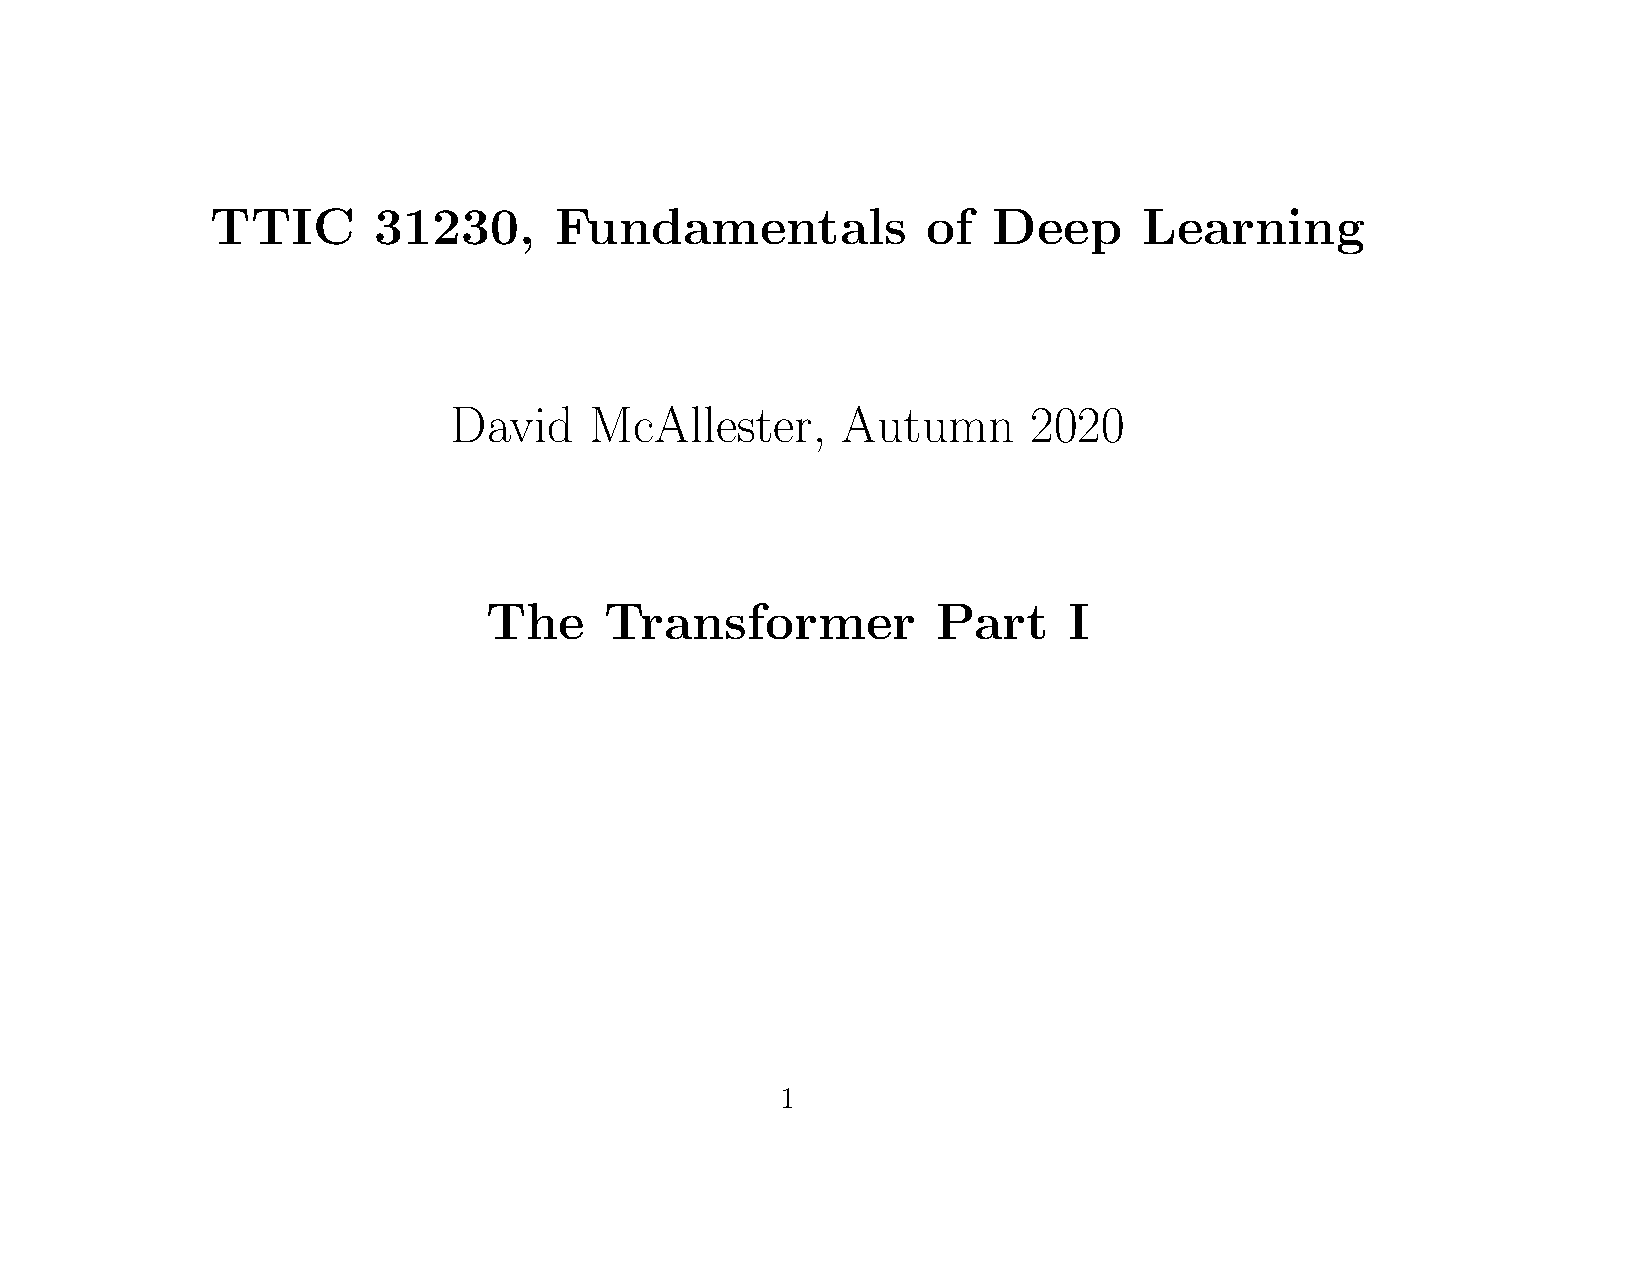
\includegraphics[height=4.5in]{\images/transformer}}

{\huge
\centerline{Jay Alammar's blog}
}

Position encodings are inserted at the bottom.

\slide{Encoding Positional Information}

At the input layer we augment the word embeddings with position information. For example:

\vfill
{\color{red} $$h[0,t,J] = e[w[t],I];e^{i\omega t}\;;e^{i2\omega t}\;;e^{i4\omega t}\cdots;e^{i2^k\omega t}$$}

\vfill
In modern versions a position encoding is trained for each position in the text.

\slide{ELMO: Language Modeling}

To do language modeling we fix $\alpha[k,t_1,t_2] = 0$ for $t_2 > t_1$.

\vfill
We can then predict the word $w_t$ as

\vfill
$$P(w_t|w_1,\ldots,w_{t-1}) = \softmax_{w_t}\;e[w_t,I]h_\mathrm{top}[t-1,I]$$

\vfill
where $h_\mathrm{top}$ is the top level hidden vector of the transformer.

\slide{Machine Translation}

Translation is just a conditional language model.

\vfill
We take the input English sentence followed by a special token and then generate the output from the transformer language model.

\slide{Continuing from a Prompt}


GPT-2 from Open AI.

\vfill
{\color{red} Continue from:}

\vfill
In a shocking finding, scientist discovered a herd of unicorns living in a remote, previously unexplored valley, in the Andes Mountains. Even more surprising to the researchers was the fact that the unicorns spoke perfect English.

\slide{The Predicted Continuation}

{\color{red} Continuation excerpted from a single response, the response selected from 10 tries.}

\bigskip

The scientist named the population, after their distinctive horn, Ovid’s Unicorn. These four-horned, silver-white unicorns were previously unknown to science.

Now, after almost two centuries, the mystery of what sparked this odd phenomenon is finally solved.

Dr. Jorge Pérez, an evolutionary biologist from the University of La Paz, and several companions, were exploring the Andes Mountains when ...
Pérez and his friends were astonished to see the unicorn herd. ...
While examining these bizarre creatures the scientists discovered that the creatures also spoke some fairly regular English. Pérez stated, “We can see, for example, that they have a common ‘language,’ something like a dialect or dialectic.”

Dr. Pérez believes that the unicorns may have originated in Argentina ... some believe that perhaps the creatures were created when a human and a unicorn met each other in a time before human civilization. ... However, Pérez also pointed out that it is likely that the only way of knowing for sure if unicorns are indeed the descendants of a lost alien race is through DNA. ...

\slide{END}

}
\end{document}
